% Results — complete, all figures, [H] placement
\section{Experimental Results}

\subsection{Experimental Setup}

Four variants stress different robustness aspects: Pure (128/32 train/test, single-device), Noise (960/240, four concurrent devices), Normal (1,802/451, all original samples), Augmented ($\sim$9,875/$\sim$240, synthetic training). All models use 5-fold stratified CV, 80/20 splits; primary metric MCC~\cite{chicco2020mcc,chicco2023mcc}. Seed~42 unless noted.

\subsection{Variant-Level Comparison}

Figure~\ref{fig:variant_mcc} shows best MCC per variant. Pure yields RNN 0.881 (seed~3). Noise degrades to DS~RNN\_B 0.798 (9.4\% drop). Normal reaches DeepStackEnsemble 0.859; augmentation lifts HPO~TCN to 0.865. Vs.~classical ML~\cite{ribeiro2026eucnc} (GP 0.756 combined, KNN 0.922 pure, CatBoost 0.770 noise): DL improves combined ($+$13.6\%) and noise ($+$3.6\%), but trails on pure ($-$4.4\%) where 128 samples are insufficient.

\begin{figure}[H]
\centering
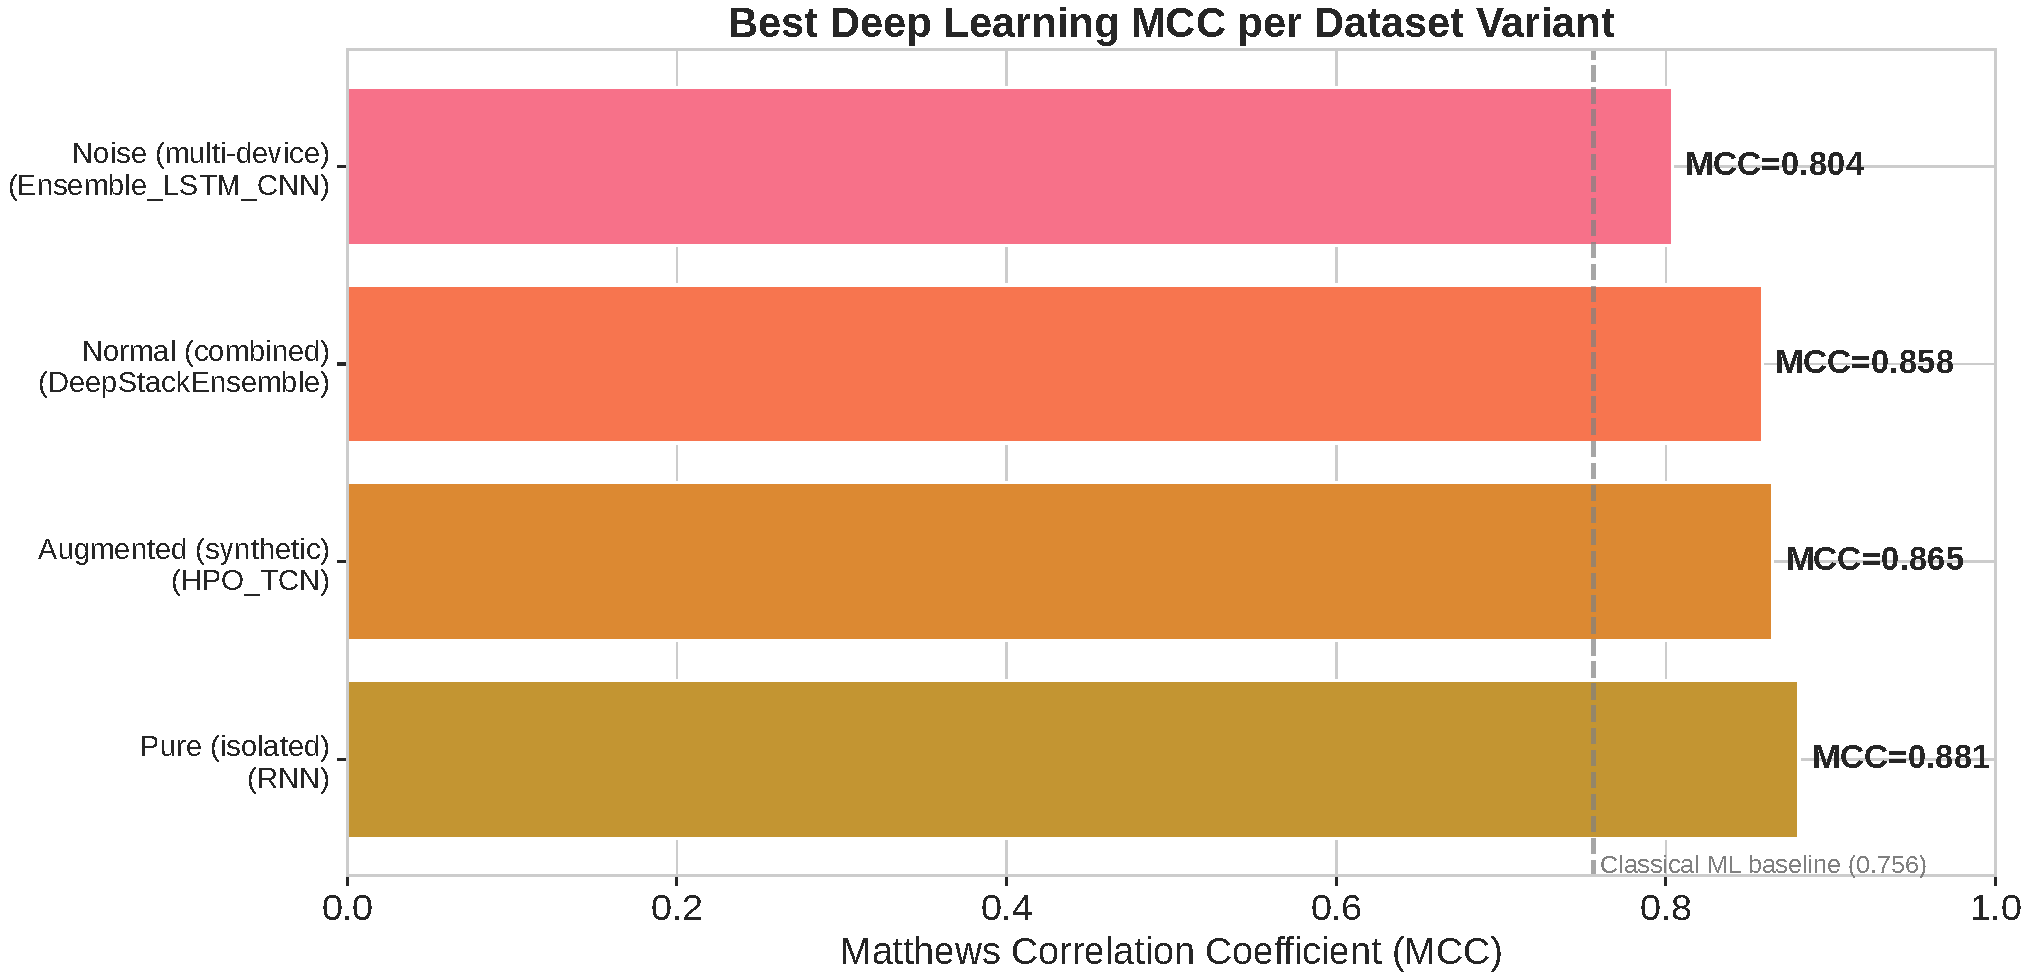
\includegraphics[width=0.80\columnwidth]{images/variant_mcc_comparison.pdf}
\caption{Best model MCC per variant. Classical baseline (0.756) dashed.}
\label{fig:variant_mcc}
\end{figure}

\subsection{Architecture Performance and HPO}

CNN (MCC 0.838) and TCN (0.836) lead single architectures; recurrent defaults underperform (RNN 0.755, GRU 0.710). Mamba (0.800) beats Transformer (0.713) by 12.2\% with $O(L)$ complexity. HPO yields large recurrent gains: GRU 0.710$\to$0.852 ($+$20.0\%), LSTM 0.686$\to$0.844 ($+$23.1\%), BiLSTM 0.684$\to$0.820 ($+$19.9\%). CNN/TCN gain less. Each model underwent 100 Optuna TPE trials; SoftMoE used NSGA-II.

Table~\ref{tab:combined_results} lists top models. DeepStackEnsemble (18 base models $\to$ per-class Level2Net $\to$ residual MetaMLP) achieves best combined MCC 0.859. Voting pairs improve over individuals (CNN$+$TCN 0.859 augmented); adding weaker models degrades (All-9: 0.807).

\begin{table}[H]
\centering
\caption{Top Models by Variant}
\label{tab:combined_results}
\resizebox{\columnwidth}{!}{\begin{tabular}{@{}lccc@{}}\toprule
\textbf{Model} & \textbf{Variant} & \textbf{MCC} & \textbf{Acc.} \\\midrule
DeepStackEnsemble  & Normal    & 0.8585 & 0.8937 \\
HPO GRU            & Normal    & 0.8524 & 0.8893 \\
HPO TCN            & Normal    & 0.8470 & 0.8843 \\
CNN                & Normal    & 0.8383 & 0.8774 \\\midrule
HPO TCN            & Augmented & 0.8647 & 0.8982 \\
HPO CNN            & Augmented & 0.8642 & 0.8977 \\
Ensemble CNN$+$TCN & Augmented & 0.8587 & 0.8932 \\\midrule
RNN                & Pure\textsuperscript{*}   & 0.8808 & 0.9063 \\\midrule
DS RNN\_B          & Noise\textsuperscript{*}  & 0.7981 & 0.8458 \\
HPO LSTM           & Noise\textsuperscript{*}  & 0.7908 & 0.8417 \\\bottomrule
\multicolumn{4}{c}{\footnotesize\textsuperscript{*}Seed~3.}\end{tabular}}
\end{table}

\subsection{Per-Class Performance}

Per-class F1 reveals consistent difficulty patterns. AB (alighting) leads (F1 0.893--0.925) due to distinctive descending trajectory; AA (inside) is hardest (0.831--0.894) from signal saturation near the AP; BB (at stop, 0.818--0.907) benefits from low RSSI; BA (boarding, 0.838--0.914) has moderate difficulty. Noise degrades AB most because concurrent near-AP transmissions mask its 20~dBm descent.

Figure~\ref{fig:cm} shows confusion matrices for the two best single-classification approaches. DeepStackEnsemble classifies 89.3\% correctly, with AA$\leftrightarrow$BA (both near-AP states) and AB$\leftrightarrow$BB (both exterior locations) as primary confusion pairs. CNN shows a qualitatively similar pattern with more off-diagonal errors, particularly misclassifying AA as AB near the AP.

\begin{figure}[H]
\centering
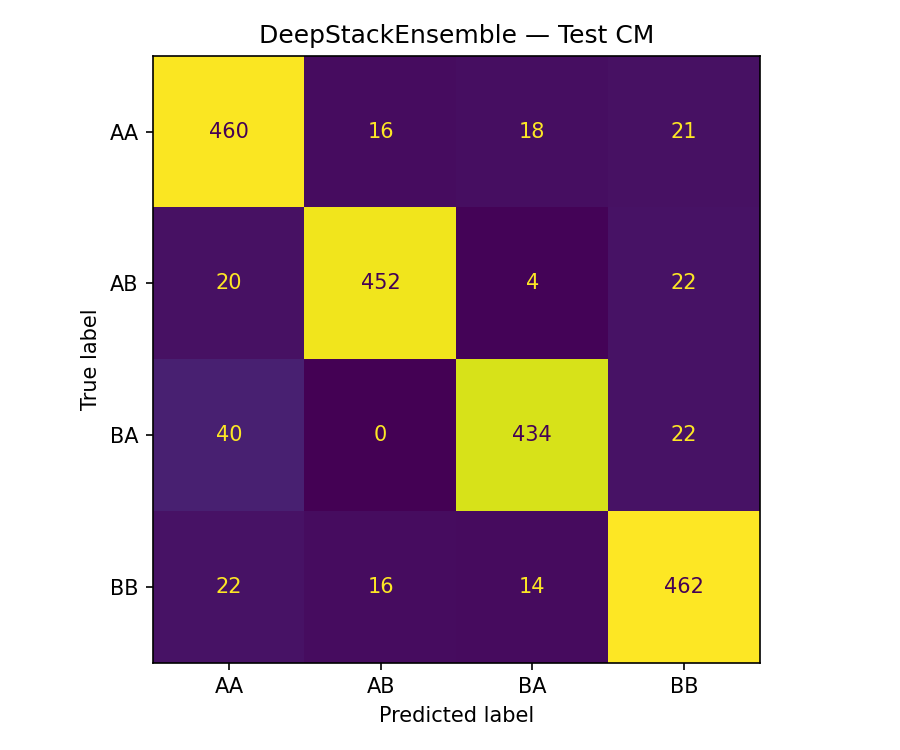
\includegraphics[width=0.42\textwidth]{images/cm_deepstack.png}\hfill
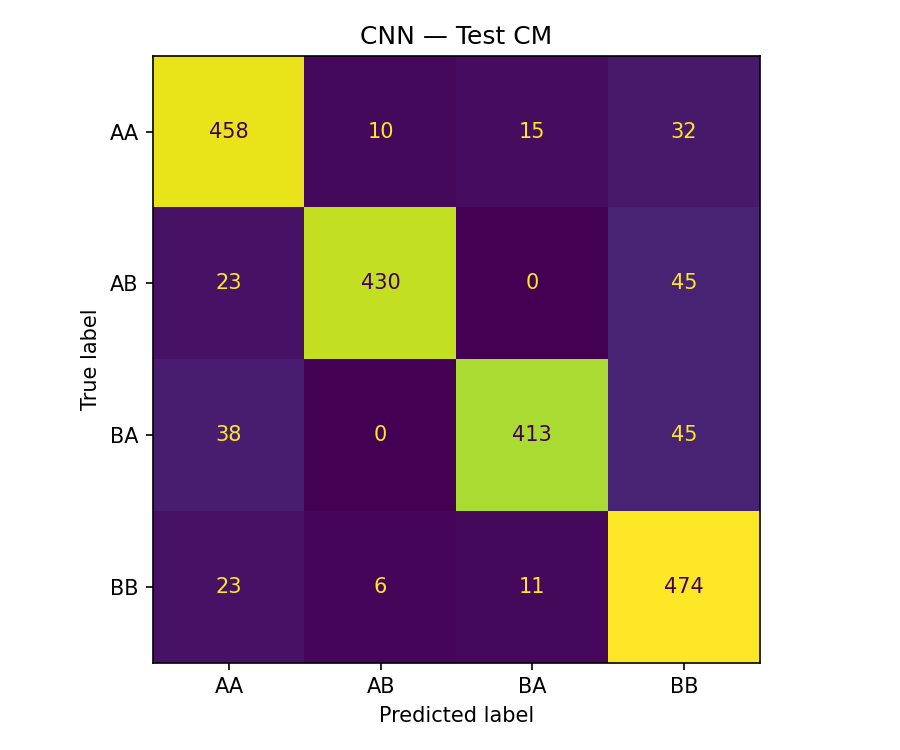
\includegraphics[width=0.42\textwidth]{images/cm_cnn.png}
\caption{Confusion matrices: DeepStackEnsemble (left, MCC 0.859) and CNN (right, MCC 0.838).}
\label{fig:cm}
\end{figure}

\subsection{Noise and Interference Analysis}

Figure~\ref{fig:interference_heatmap} quantifies mean RSSI shift per (Route $\times$ Interferer) pair. Three patterns emerge: (1) AA dominates as interferer ($+$45--53~dBm) because devices near the AP transmit at high power; BB causes minimal shift ($\le +$3.1~dBm). (2) AB is most affected ($+$46.6~dBm from AA): near-AP transmissions mask its descent. (3) Self-interference is minimal ($+$1.2--4.6~dBm).

\begin{figure}[H]
\centering
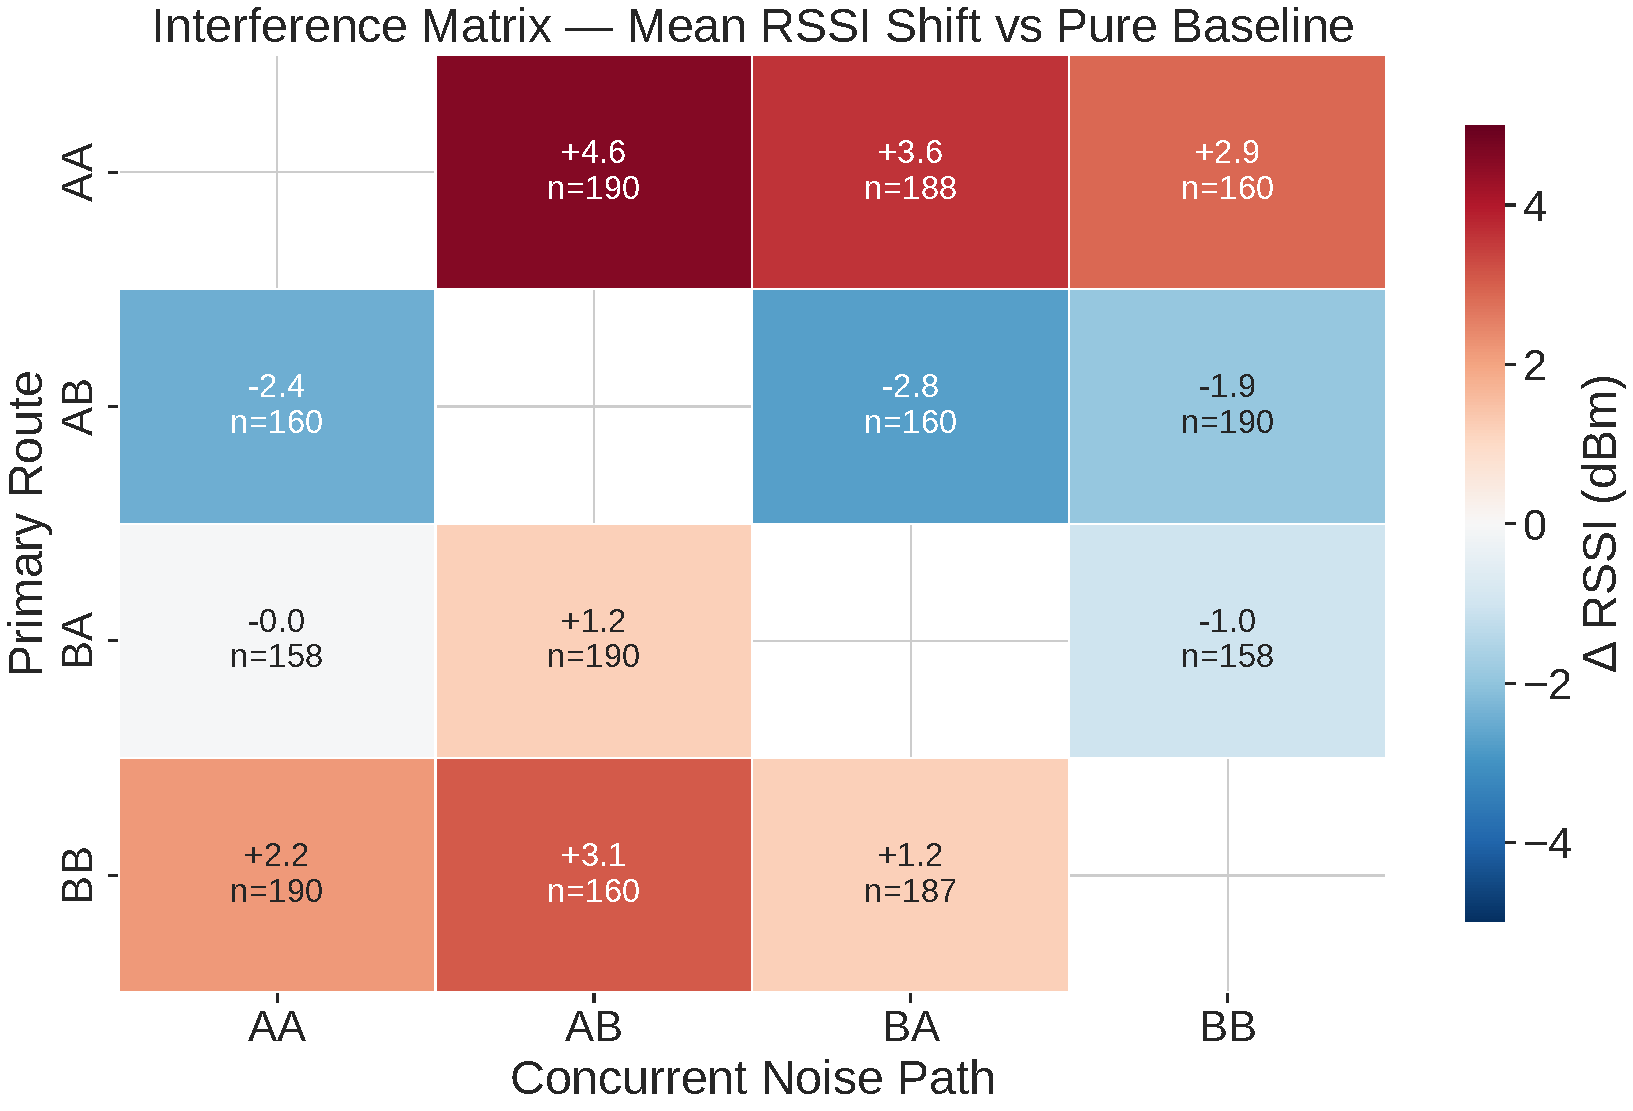
\includegraphics[width=0.85\columnwidth]{images/interference_heatmap.pdf}
\caption{Interference heatmap: AA dominates; self-interference minimal.}
\label{fig:interference_heatmap}
\end{figure}

Figure~\ref{fig:trajectories} explains \emph{why} each class degrades differently under interference. AA suffers from BA raising its stable high-RSSI profile, making near-AP states hard to separate. AB's 20~dBm descent is flattened by AA into a constant profile indistinguishable from AA---directly explaining AB's noise-induced F1 drop. BA's ascending trajectory is compressed by AA interference, reducing the distinctive 15~dBm ascent. BB's flat $-$50~dBm pattern shifts upward under AA but retains its shape, explaining BB's noise resilience: classification depends on temporal flatness, not absolute level.

\begin{figure}[H]
\centering
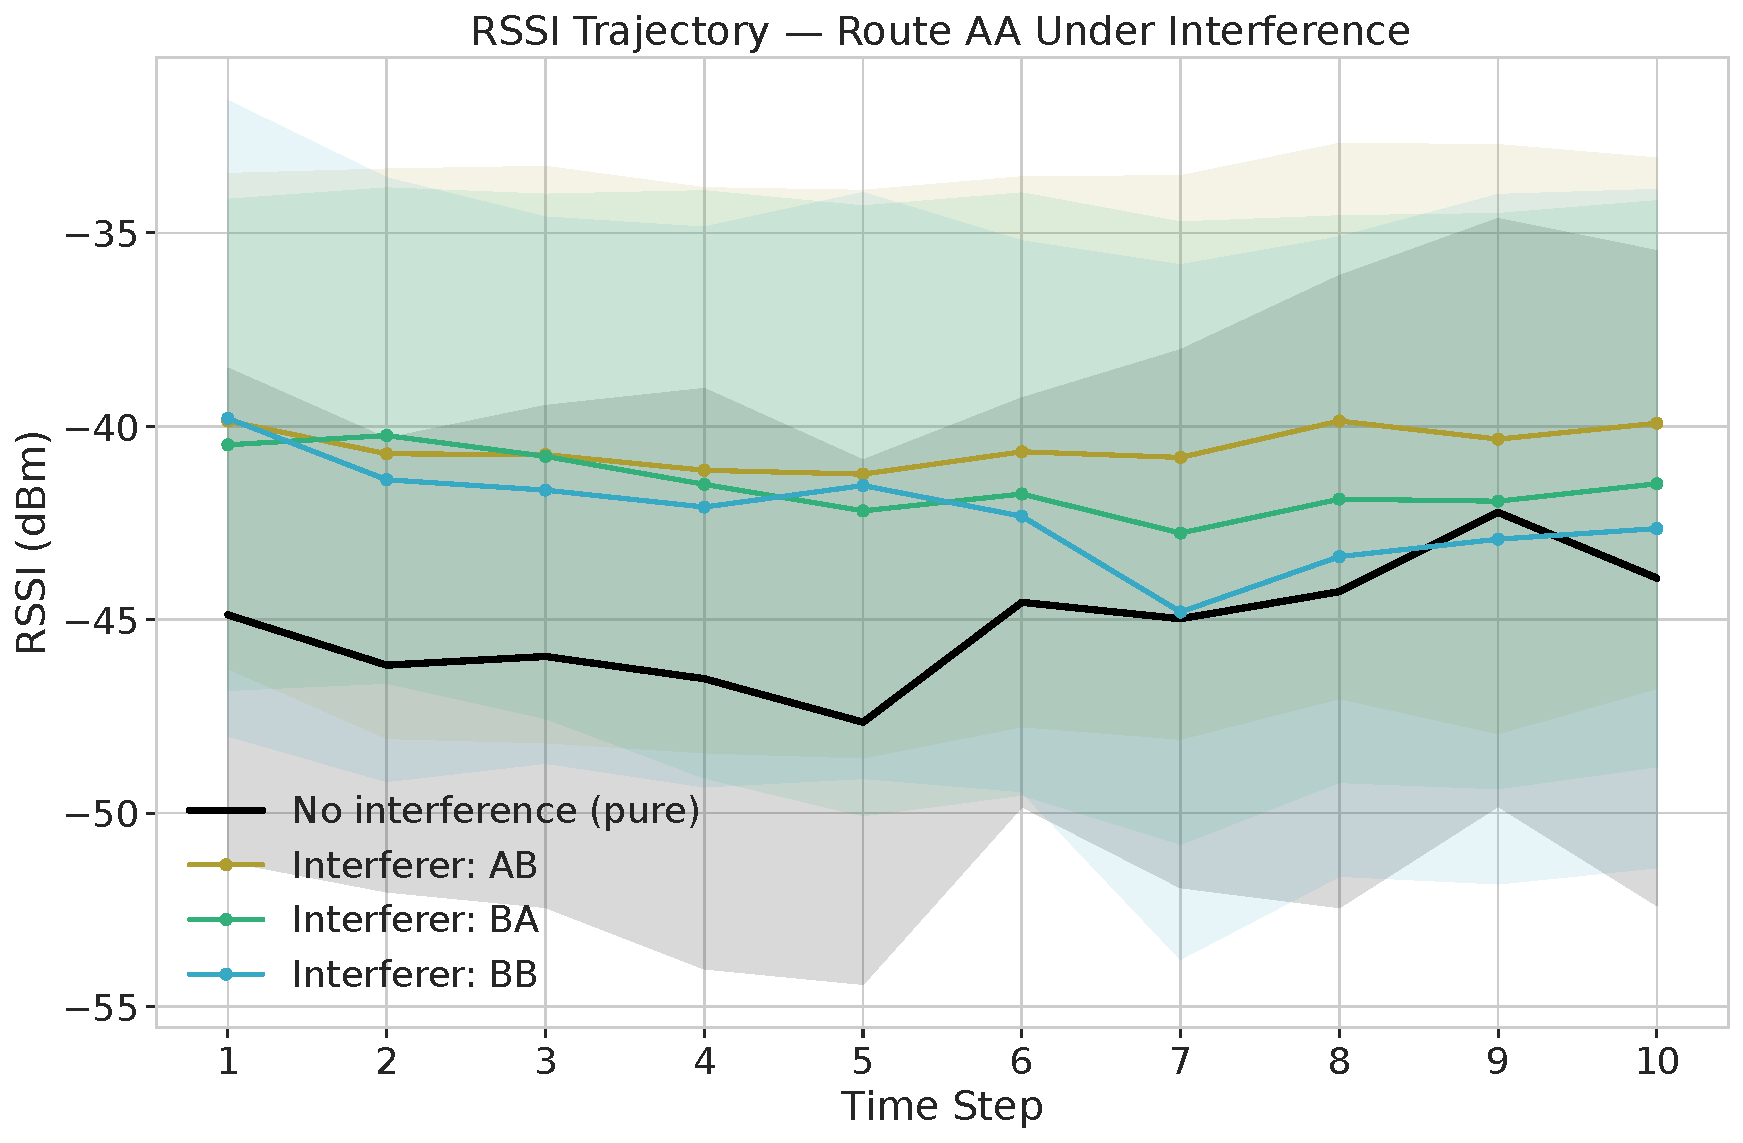
\includegraphics[width=0.45\textwidth]{images/interference_trajectory_AA.pdf}\hfill
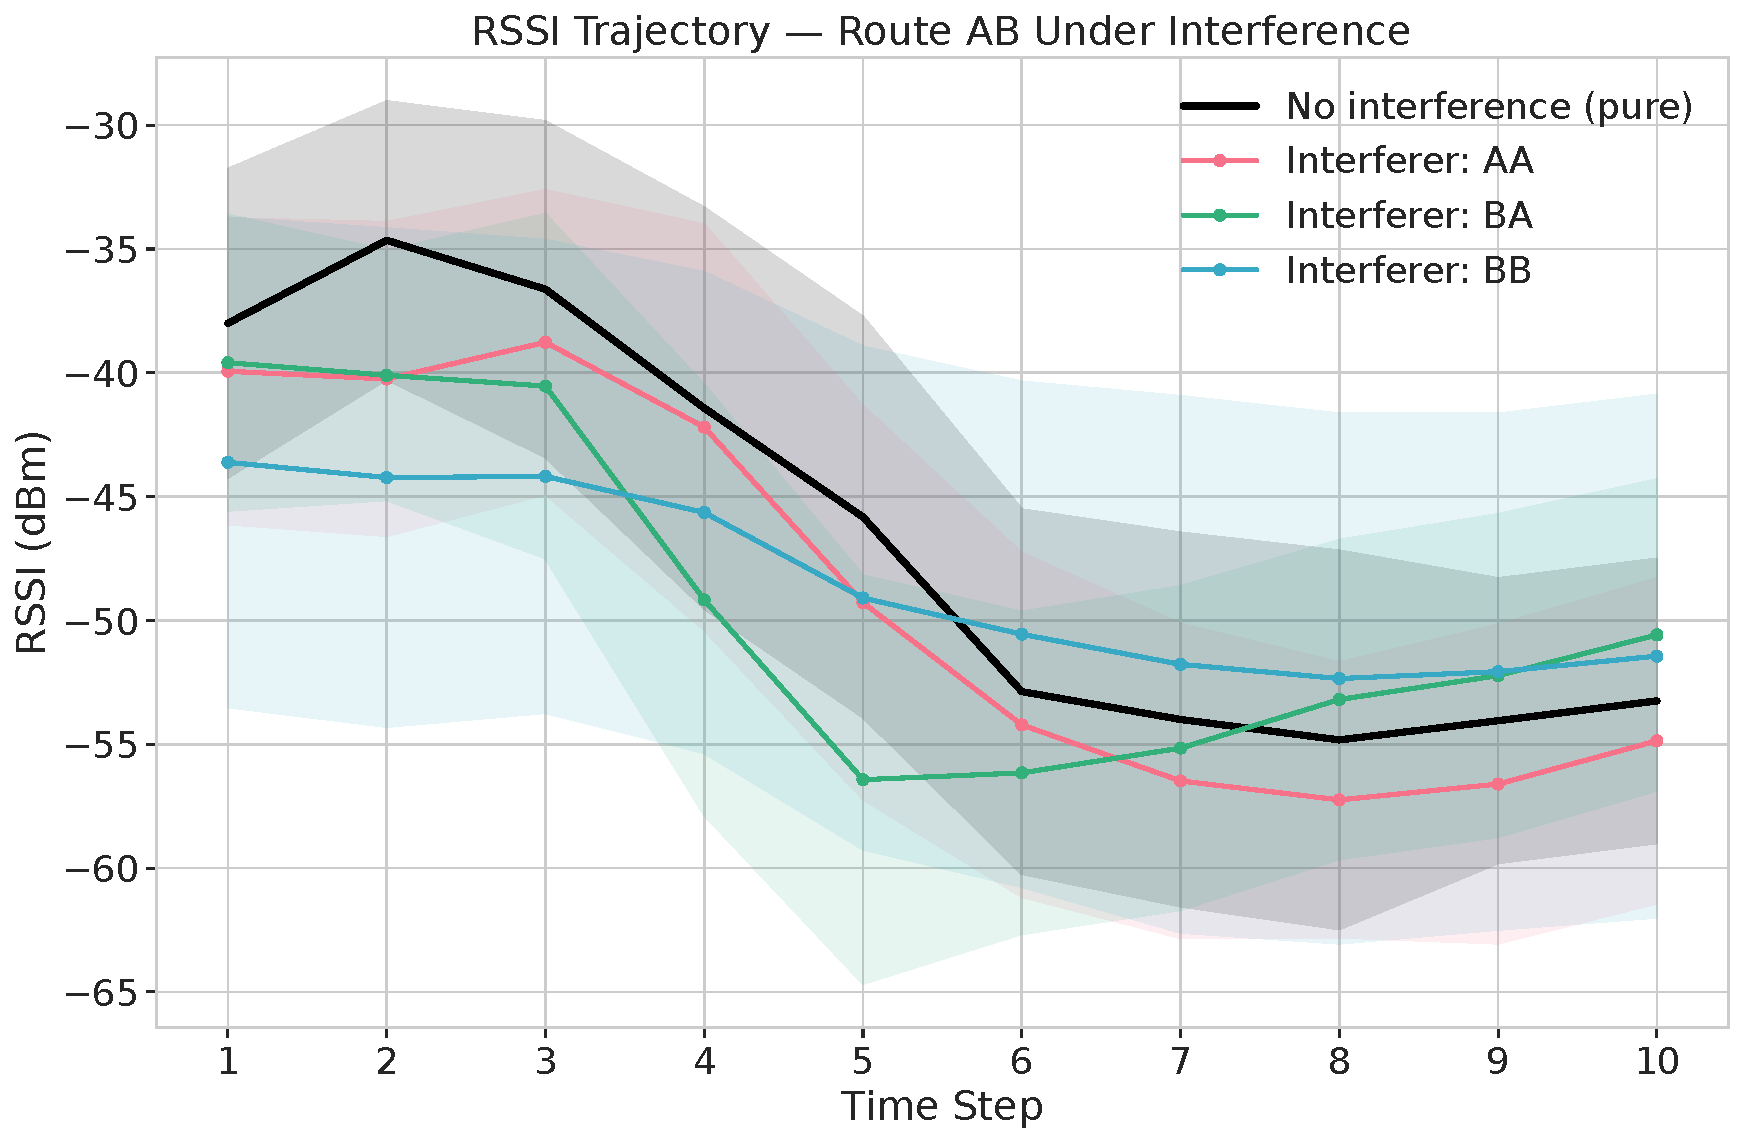
\includegraphics[width=0.45\textwidth]{images/interference_trajectory_AB.pdf}\\[4pt]
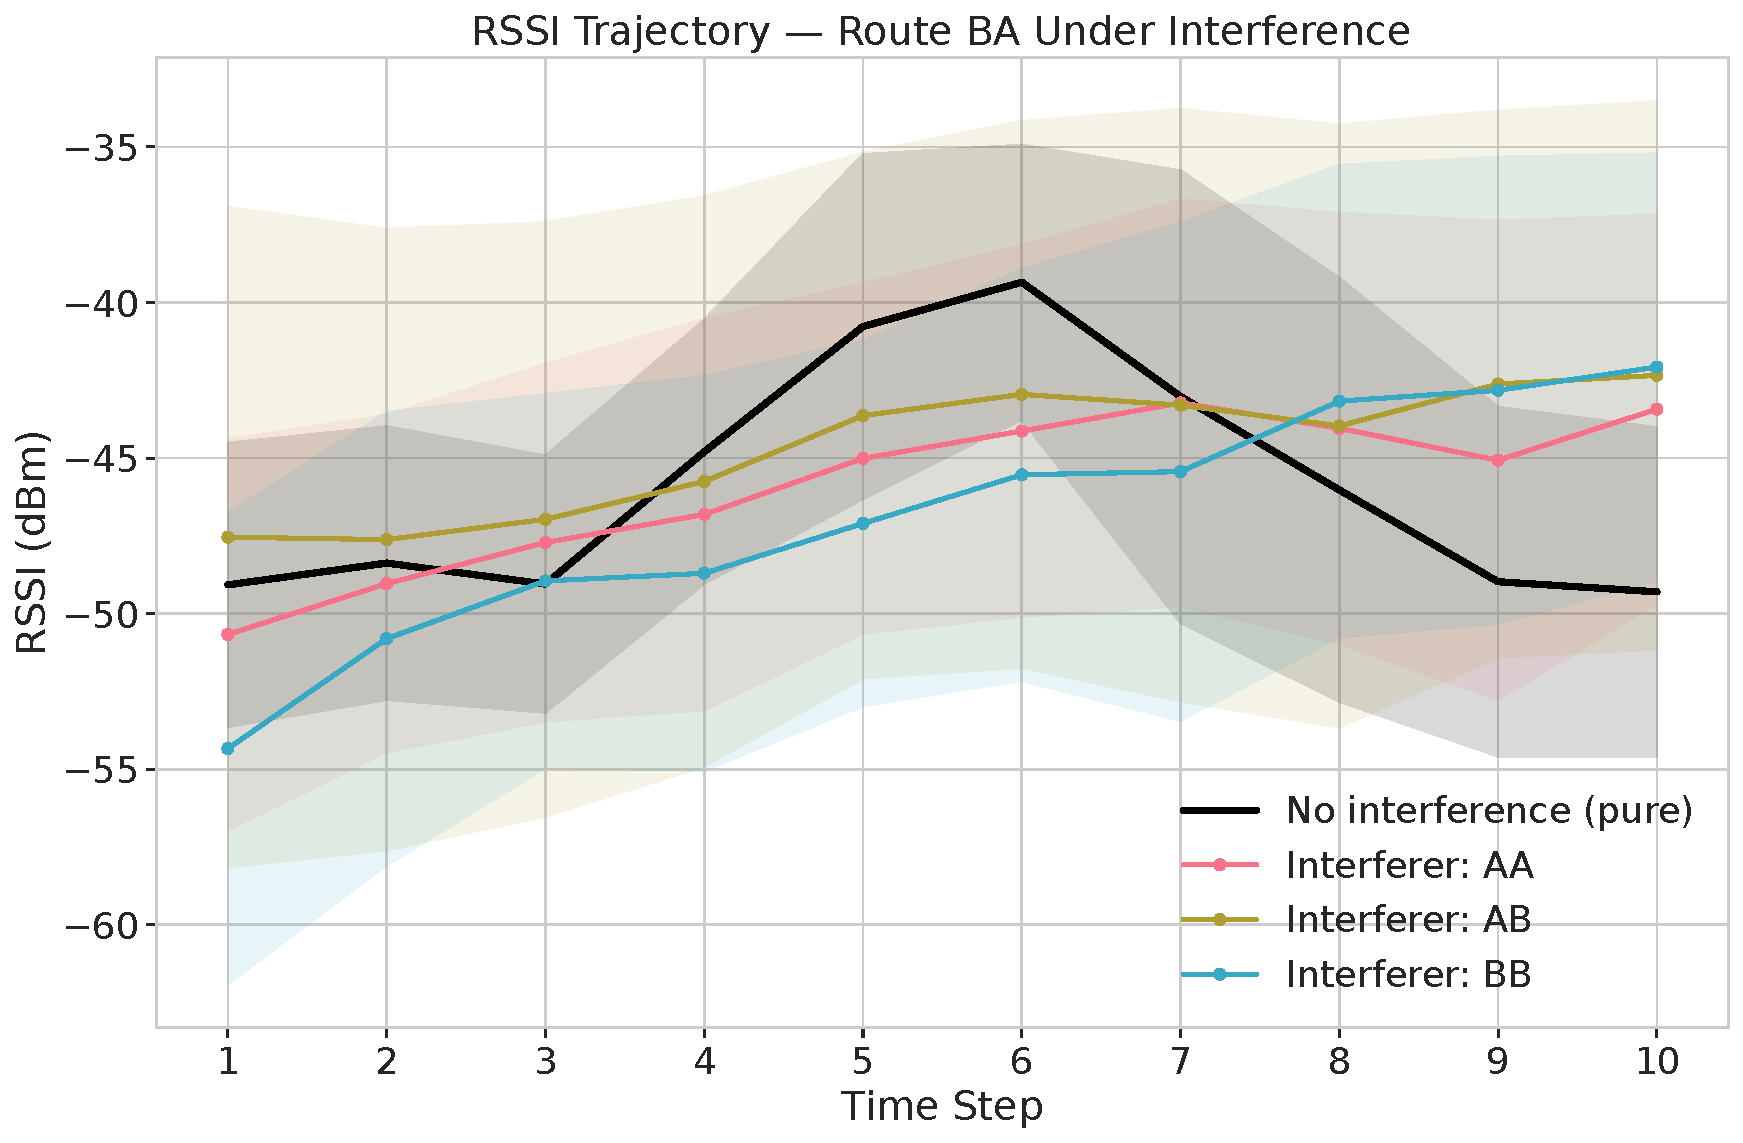
\includegraphics[width=0.45\textwidth]{images/interference_trajectory_BA.pdf}\hfill
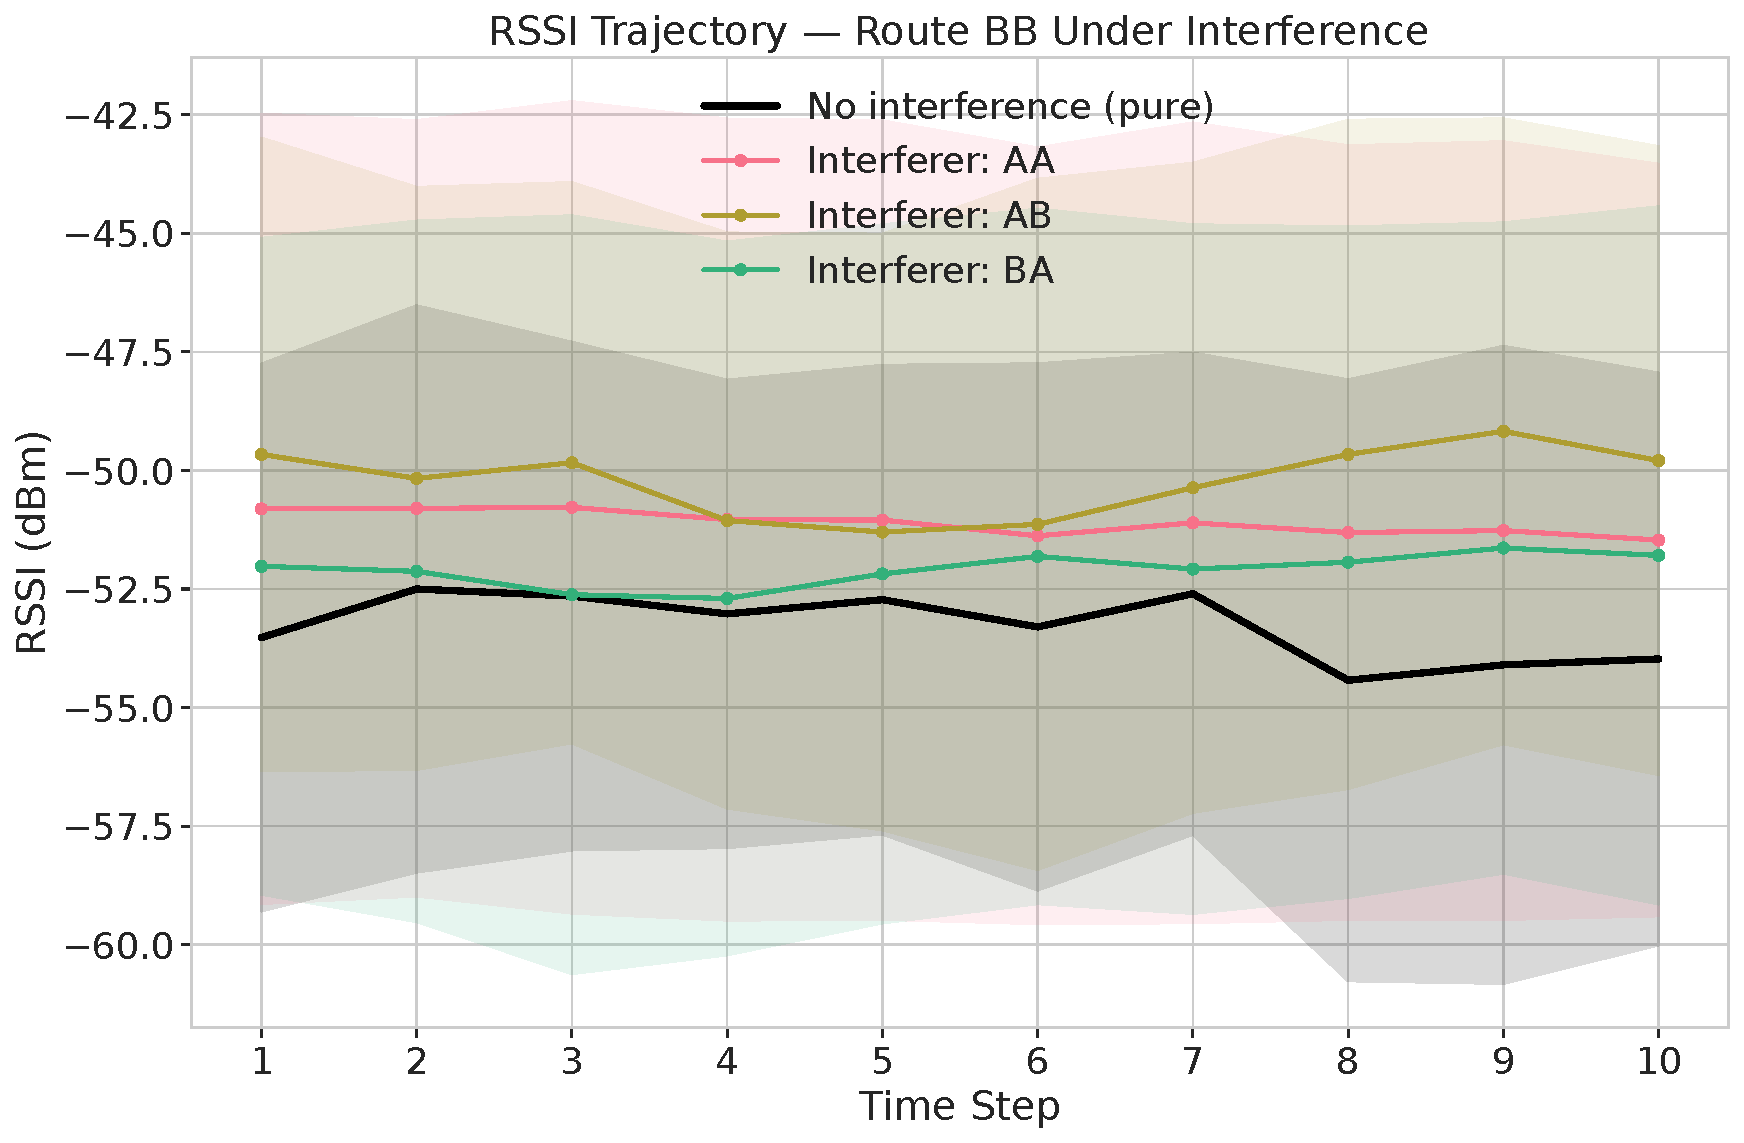
\includegraphics[width=0.45\textwidth]{images/interference_trajectory_BB.pdf}
\caption{Trajectories under interference. Top-left: AA---BA raises profile. Top-right: AB---AA masks descent entirely. Bottom-left: BA---AA compresses ascent. Bottom-right: BB---flat pattern persists despite shift.}
\label{fig:trajectories}
\end{figure}

Per-timestep analysis reveals perturbation peaks at timesteps~4--6 (closest to AP). MetaFusion\_GRU reaches MCC 0.783 on noise (vs.~0.758 for standard GRU) by encoding noise context, though the gap to pure (0.881) confirms that metadata alone cannot fully compensate for signal ambiguity under concurrent transmissions.

CNN (28K params, 129~s) offers the best efficiency-accuracy tradeoff among single models. Mamba (89K, 374~s) provides $O(L)$-complexity competitive accuracy. HPO GRU (198K, 107~s) is the strongest single model. DeepStackEnsemble (1.2M) suits server-side deployment.

\subsection{Feature Importance}

Permutation importance analysis across the 4 engineered channels and 10 timesteps, averaged over CNN, TCN, and GRU, reveals that window deviation---how far each timestep deviates from the per-sample mean---is the most informative channel (mean $\Delta$MCC $9.1\times 10^{-3}$), particularly at early timesteps ($t\!=\!1$--3) where it captures each class's characteristic offset from its baseline. This confirms that trajectory shape, not absolute magnitude, carries the strongest discriminative signal.

Velocity ($\Delta$) peaks at $t\!=\!4$ ($18.4\times 10^{-3}$), the mid-trajectory moment of maximum movement. Raw RSSI matters most at $t\!=\!6$, where absolute levels separate near-AP from exterior positions. Acceleration ($\Delta^2$) contributes at $t\!=\!3$--5, capturing directional movement onset. These results validate the 4-channel engineering strategy and align with the trajectory analysis in Figure~\ref{fig:trajectories}, where AB's defining 20~dBm descent occurs during timesteps~4--7.

\begin{figure}[H]
\centering
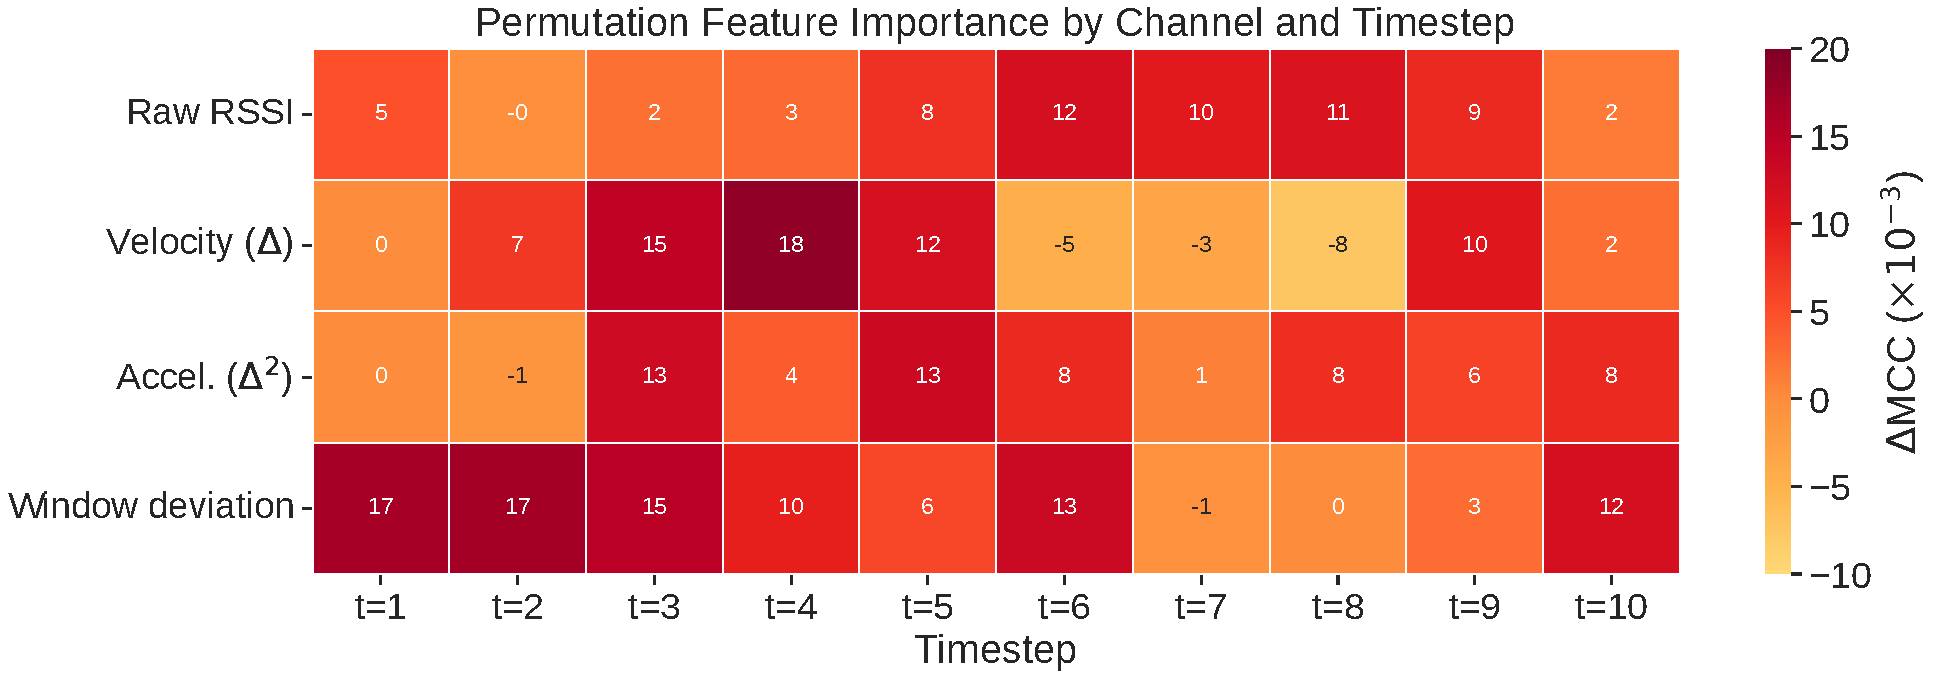
\includegraphics[width=0.85\columnwidth]{images/feature_importance_dl.pdf}
\caption{Permutation feature importance ($\Delta$MCC) across 4 channels $\times$ 10 timesteps, averaged over CNN, TCN, and GRU.}
\label{fig:feature_importance}
\end{figure}
